% User guide for the primate vocalization detector: viewer.exe (GUI) and detect.exe (console).
% The screenshots in fig/ are generated from the viewer itself by docs/manual/screenshots.py.
%
%   make manual            -> docs/manual/build/manual.pdf
%
\documentclass[11pt,a4paper]{article}

\usepackage[utf8]{inputenc}
\usepackage[T1]{fontenc}
\usepackage{lmodern}
\usepackage[english]{babel}
\usepackage{microtype}
\usepackage[a4paper,margin=2.5cm]{geometry}
\usepackage{graphicx}
\usepackage{xcolor}
\usepackage{booktabs}
\usepackage{tabularx}
\usepackage{array}
\usepackage{enumitem}
\usepackage{parskip}
\usepackage{fancyvrb}
\usepackage{float}
\usepackage{needspace}
\usepackage{tikz}
\usepackage[os=win]{menukeys}
\usepackage[font=small,labelfont=bf,skip=6pt]{caption}
\usepackage{titlesec}
\usepackage[hidelinks]{hyperref}

\graphicspath{{fig/}}

\newcommand{\version}{0.1.5}
\newcommand{\viewer}{\texttt{viewer.exe}}
\newcommand{\detect}{\texttt{detect.exe}}
\newcommand{\ui}[1]{\textsf{\textbf{#1}}}
\newcommand{\file}[1]{\texttt{#1}}
\newcommand{\shot}[1]{\includegraphics[width=\textwidth]{#1}}

\hypersetup{
  pdftitle  = {Primate Vocalization Detector: User Guide},
  pdfauthor = {Fernando Nelson Candia Aroni},
  pdflang   = {en}
}
\titleformat*{\section}{\Large\bfseries\raggedright}
\titleformat*{\subsection}{\large\bfseries\raggedright}
\setlist{nosep}
\setlist[enumerate]{itemsep=3pt}
\setlist[itemize]{itemsep=3pt}
\definecolor{callout}{HTML}{1E66F5}
\tikzset{callout/.style={circle,fill=callout,text=white,font=\bfseries\small,inner sep=2pt,minimum size=16pt}}
\newcommand{\callout}[1]{\tikz[baseline=-3.5pt]{\node[callout]{#1};}}
% A shortcut never breaks across lines.
\let\menukeyskeys\keys
\renewcommand{\keys}[1]{\mbox{\menukeyskeys{#1}}}

\begin{document}

\begin{titlepage}
  \centering
  \vspace*{3cm}
  {\Huge\bfseries Primate Vocalization\\[4pt] Detector\par}
  \vspace{1cm}
  {\LARGE User Guide\par}
  \vspace{2cm}
  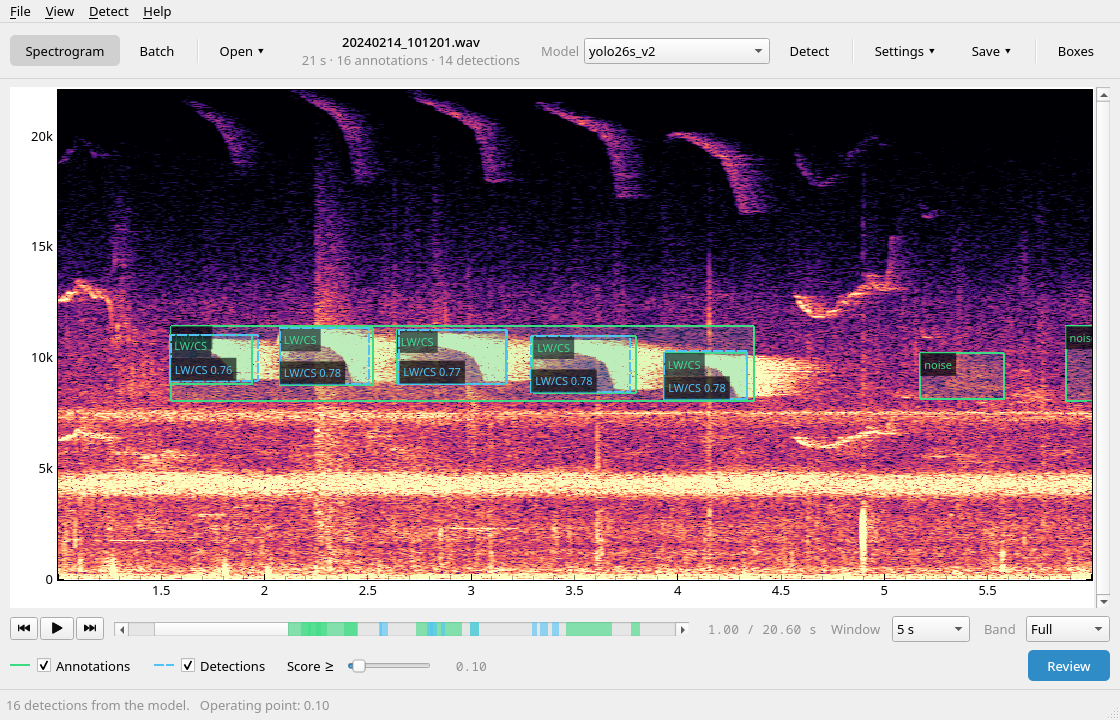
\includegraphics[width=0.85\textwidth]{spectrogram}
  \vfill
  {\large Version \version{} · Windows 10/11, 64-bit\par}
  \vspace{0.4cm}
  {\small Fernando Nelson Candia Aroni · Pontificia Universidad Católica del Perú\par}
\end{titlepage}

\tableofcontents
\clearpage

% =====================================================================
\section{Introduction}

The program finds monkey calls in audio recordings. It draws a \emph{box} around each call
on the spectrogram and tells you the species, the call type and a \emph{score} (how sure it
is).

The boxes are saved as a \textbf{Raven selection table}: a text file that opens in Raven Pro,
Excel or the program itself. For a recording \file{name.wav} you get \file{name.detections.txt}
next to it.

You get two programs:

\begin{itemize}
  \item \viewer{} --- the window. Open a recording, run the model, listen, review the boxes
    one by one, process a whole folder.
  \item \detect{} --- the command line. Process folders without a window, or from a script.
\end{itemize}

% =====================================================================
\section{Installation}

\begin{enumerate}
  \item Download from \url{https://github.com/nhrot-fc/tesis-primate/releases}:
    \begin{itemize}
      \item \file{detector-\version-win64-cpu.zip} (any PC) \textbf{or}
        \file{detector-\version-win64-cuda.zip} (PC with an NVIDIA graphics card);
      \item at least one model: \file{detector-\version-model-\emph{name}.zip}.
    \end{itemize}
  \item Unzip the \file{win64} zip into a short path, for example
    \file{C:\textbackslash detector\textbackslash}.
  \item Unzip the model zip into \textbf{the same folder}, next to \viewer{}.
\end{enumerate}

Nothing else to install: Python and all the libraries are inside. No internet needed.

\begin{center}
\begin{tabular}{@{}ll@{}}
  \toprule
  Windows & 10 or 11, 64-bit \\
  Memory & 8 GB (16 GB with a graphics card) \\
  Disk & 3 GB free (\file{cpu}) or 7 GB (\file{cuda}) \\
  Graphics card & optional; NVIDIA with 4 GB and driver 570 or newer \\
  \bottomrule
\end{tabular}
\end{center}

% =====================================================================
\section{Execution}

Double-click \viewer{}. To open a recording right away, drag it onto \viewer{}.

The first time:

\begin{itemize}
  \item Windows says \emph{Windows protected your PC}. Click \ui{More info}, then
    \ui{Run anyway}. It happens only once.
  \item The launch is slow: the antivirus checks the new files.
\end{itemize}

Every time:

\begin{itemize}
  \item The status bar says \emph{Loading detection engine} for a few seconds. You can open
    a recording meanwhile. \ui{Detect} turns on when it says \emph{Ready}.
  \item If the program does not open, read \file{viewer.log}, next to \viewer{}.
\end{itemize}

For the command line, see section~\ref{sec:cli}.

% =====================================================================
\section{Adding a model}

A model is a folder inside \file{models\textbackslash}. There are three models: Faster R-CNN
(most accurate, slowest), YOLO26s (fastest) and AST-Deformable DETR (in between).

\begin{enumerate}
  \item Download its zip, \file{detector-\version-model-\emph{name}.zip}.
  \item Unzip it into the program folder (next to \viewer{}), or just drop the zip on the
    program's window.
  \item Pick it in the \ui{Model} list of the toolbar.
\end{enumerate}

With one model installed, it is already picked.

% =====================================================================
\section{Viewer}

\subsection{The window}

\begin{figure}[H]
  \centering
  \begin{tikzpicture}
    \node[anchor=south west,inner sep=0] (img) {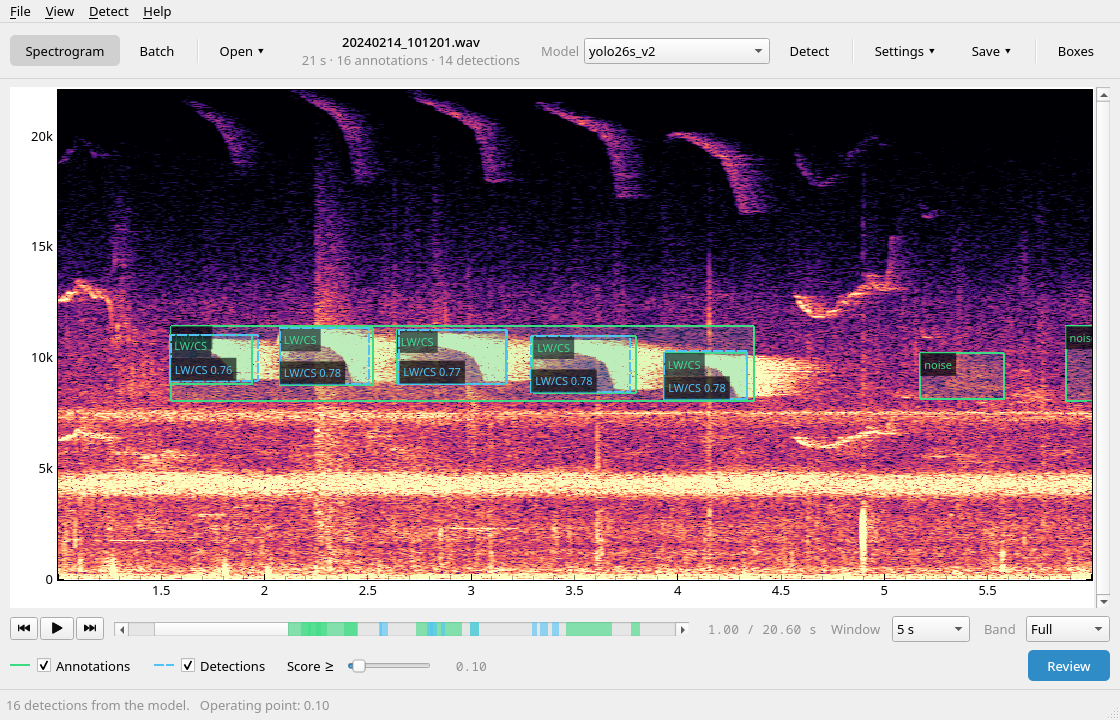
\includegraphics[width=0.9\textwidth]{spectrogram}};
    \begin{scope}[x={(img.south east)},y={(img.north west)}]
      \node[callout] at (-0.025,0.983) {1};
      \node[callout] at (-0.025,0.93)  {2};
      \node[callout] at (-0.025,0.52)  {3};
      \node[callout] at (-0.025,0.127) {4};
      \node[callout] at (-0.025,0.075) {5};
      \node[callout] at (-0.025,0.02)  {6};
    \end{scope}
  \end{tikzpicture}
  \caption{A recording with annotations (green) and detections (blue, with score).}
\end{figure}

\begin{enumerate}[label=\protect\callout{\arabic*}, leftmargin=*]
  \item \textbf{Menus.} Everything the program does, with its keyboard shortcut.
  \item \textbf{Toolbar.} The two views (\ui{Spectrogram}, \ui{Batch}), \ui{Open}, the
    open recording, the \ui{Model}, \ui{Detect}, \ui{Settings}, \ui{Save}, \ui{Boxes}.
    The blue button is always the next step.
  \item \textbf{Spectrogram.} Time left to right, frequency bottom to top.
  \item \textbf{Transport.} Play, the time bar (the marks are the boxes), \ui{Window} (how
    many seconds you see) and \ui{Band} (how many Hz you see).
  \item \textbf{Score and Review.} Appears when there are detections.
  \item \textbf{Status bar.} What just happened, and what is running.
\end{enumerate}

\subsection{Open a recording}

Drag a WAV, FLAC or MP3 file onto the window, or \menu{File > Open audio\ldots}
(\keys{\ctrl+O}).

If the recording already has a \file{.detections.txt} next to it, it opens too.

To see a Raven table made by hand: \menu{File > Open annotations\ldots} (\keys{\ctrl+T}).
It shows in green.

\subsection{Detect}

\begin{enumerate}
  \item Press \ui{Detect} (\keys{\ctrl+R}).
  \item Wait. The status bar shows the progress.
  \item The boxes appear in blue with their score.
\end{enumerate}

\begin{figure}[H]
  \centering
  \shot{context}
  \caption{Below the spectrogram: the layers, the \ui{Score} filter and \ui{Review}.}
\end{figure}

\ui{Score $\geq$} hides the boxes with a lower score. It starts at the best value for the
model. Move it left to see more boxes, right to see fewer.

\ui{Boxes} (\keys{\ctrl+E}) opens the list of boxes. Click a row to go to that box. Press
\keys{Del} to remove it.

\subsection{Review}

\ui{Review} shows the detections one at a time so you can check them.

\begin{figure}[H]
  \centering
  \shot{review}
  \caption{Review: the box is zoomed in and has handles.}
\end{figure}

For each box:

\begin{itemize}
  \item Press \keys{Space} to hear it.
  \item Drag the box or its corners if it is not well placed.
  \item Change the \ui{Label} if the species or call is wrong.
  \item Press \keys{A} to \ui{Accept} or \keys{R} to \ui{Reject}. The next box appears.
  \item \keys{N} and \keys{P} skip forward and back. \keys{Esc} leaves.
\end{itemize}

Accepted boxes go to the green layer. Your progress is saved: if you close the program, the
review continues where you left it.

\Needspace{9\baselineskip}
\subsection{Save}

\begin{itemize}
  \item \menu{File > Save annotations table\ldots}: the green boxes (accepted ones).
  \item \menu{File > Save detections table\ldots}: the blue boxes you can see.
  \item \menu{File > Save image\ldots} (\keys{\ctrl+S}): the screen as a PNG.
\end{itemize}

Tables are Raven files. In Raven Pro, open the audio and then \menu{File > Open Selection
Table}.

\subsection{Batch: a whole folder}

\begin{figure}[H]
  \centering
  \shot{batch_done}
  \caption{\ui{Batch} after a run: one file skipped (it had a table), two done.}
\end{figure}

\begin{enumerate}
  \item Click \ui{Batch} in the toolbar.
  \item Drag a folder onto the window, or \ui{Choose a folder\ldots}.
  \item Click \ui{Run}.
\end{enumerate}

Every recording gets its \file{.detections.txt}. Files that already have one are skipped
(tick \ui{Overwrite existing tables} to redo them). \ui{Stop} stops the run; finished files
are kept. Double-click a file to open it in the \ui{Spectrogram} view.

\subsection{Move and zoom}

\begin{center}
\begin{tabular}{@{}ll@{}}
  \toprule
  Mouse wheel & move in time \\
  \keys{\ctrl} + wheel, or \keys{\ctrl+1} / \keys{\ctrl+3} & zoom in time \\
  \keys{\shift} + wheel, or \keys{\ctrl+\arrowkeyup} / \keys{\ctrl+\arrowkeydown} & zoom in frequency \\
  \keys{\arrowkeyup} \keys{\arrowkeydown} & move the frequency band; \keys{F} shows all \\
  \keys{\arrowkeyleft} \keys{\arrowkeyright}, \keys{PgUp} \keys{PgDn} & step, page \\
  \keys{Home} \keys{End} & start, end \\
  \keys{N} \keys{P} & next, previous detection \\
  \keys{Space} & play / pause \\
  Click on the spectrogram & move the playhead \\
  \bottomrule
\end{tabular}
\end{center}

\keys{F1} shows all shortcuts inside the program.

% =====================================================================
\section{Detector CLI}
\label{sec:cli}

\detect{} does the same as \ui{Batch}, from the command line. Open \ui{cmd} or PowerShell in
the program folder and run:

\begin{Verbatim}[frame=single,fontsize=\small]
detect.exe --model models\yolo26s_v2 D:\recordings
\end{Verbatim}

\begin{center}
\begin{tabularx}{\textwidth}{@{}lX@{}}
  \toprule
  \file{--model} & Which model. Without it, the only installed model is used. \\
  \file{--score S} & Minimum score to keep a box. Default: the best value for the model. \\
  \file{--overwrite} & Redo files that already have a table. \\
  \file{--device cpu} & Do not use the graphics card. \\
  \bottomrule
\end{tabularx}
\end{center}

You can give several folders or files. What you see:

\begin{Verbatim}[frame=single,fontsize=\footnotesize]
Loading detection engine...
[INFO] yolo26s_v2 on cuda | score >= 0.10 | 3 recordings
[INFO] [1/3] 20240214_101201.wav already has a table; --overwrite redoes it
[INFO] [2/3] 20240214_103015.wav: 14 detections in 1 s -> 20240214_103015.detections.txt
[INFO] [3/3] 20240215_064400.wav: 14 detections in 1 s -> 20240215_064400.detections.txt
[INFO] Done. Open each audio in Raven with its .detections.txt table
\end{Verbatim}

A script that runs two folders overnight, \file{run.bat}:

\begin{Verbatim}[frame=single,fontsize=\small]
cd /d C:\detector
detect.exe --model models\frcnn D:\field\2024-02 D:\field\2024-03 > run.log
\end{Verbatim}

% =====================================================================
\section{Audio settings}

\begin{figure}[H]
  \centering
  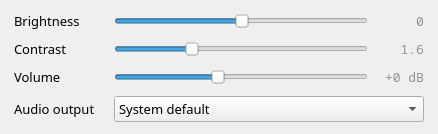
\includegraphics[width=0.55\textwidth]{settings}
  \caption{\ui{Settings}, in the toolbar.}
\end{figure}

\begin{itemize}
  \item \textbf{Audio output}: where the sound plays (speakers, headphones).
  \item \textbf{Volume}: raise it for distant calls. Field recordings are quiet.
  \item \textbf{Brightness} and \textbf{Contrast}: how the spectrogram looks.
\end{itemize}

% =====================================================================
\section{If something goes wrong}

\begin{itemize}
  \item \textbf{No sound}: \ui{Settings} $\to$ \ui{Audio output}, pick your device.
  \item \textbf{\ui{Detect} is grey}: wait for \emph{Ready} in the status bar.
  \item \textbf{No model in the list}: the model zip must be unzipped next to \viewer{},
    not inside \file{models\textbackslash}.
  \item \textbf{Very slow}: use YOLO26s, or the \file{cuda} package on a PC with an NVIDIA
    card.
  \item \textbf{The program closes}: \file{viewer.log}, next to \viewer{}, says why.
\end{itemize}

\end{document}
